\capitulo{Apresentação da solução}
\label{cap:apresentacao-solucao}

Neste capítulo, será abordada a modelagem do sistema proposto, contendo os diagramas e também os requisitos que fazem parte do trabalho.

\secao{Requisitos do Sistema}

Logo abaixo, será apresentada a tabela 3 contendo os requisitos funcionais do sistema computacional,
seguido da tabela 4 com os requisitos não funcionais do mesmo.

\begin{tabela}{Requisitos funcionais do sistema computacional}{O Autor}
\label{tab:req-funcionais}
\renewcommand{\arraystretch}{1.3}
\resizebox{\textwidth}{!}{
\begin{tabular}{|c|c|}
    \hline
    \textbf{Número Requisito} & \textbf{Requisito Funcional} \\ \hline
    01 & O sistema deve permitir a importação de vídeos contendo arremessos de basquete para análise biomecânica. \\ \hline
    02 & O sistema deve realizar a detecção da estrutura corporal do atleta nos quadros do vídeo utilizando visão computacional. \\ \hline
    03 & O sistema deve extrair dados cinemáticos dos movimentos, como ângulos articulares, posição dos membros e trajetória. \\ \hline
    04 & O sistema deve calcular a velocidade do movimento do atleta a partir da variação das posições ao longo do tempo. \\ \hline
    05 & O sistema deve apresentar graficamente os dados obtidos em tempo de execução, facilitando a análise. \\ \hline
    06 & O sistema deve identificar automaticamente o momento do arremesso para fins de segmentação do movimento. \\ \hline
\end{tabular}
}
\end{tabela}


    \begin{tabela}{Requisitos não funcionais do sistema computacional}{O Autor}
        \label{tab:req-nfuncionais}
        \resizebox{1\textwidth}{!}{
            \begin{tabular}{|c|c|}
                \hline
                \textbf{Número Requisito} & \textbf{Requisito Não Funcional}                                  \\ \hline
                01                        & O sistema computacional deve ser desenvolvido utilizando a linguagem de programação Python.                \\ \hline
                02                        & O sistema deve utilizar bibliotecas como OpenCV, MediaPipe e Matplotlib. \\ \hline
                03                        & O sistema deve ser compatível com o sistema operacionais Windows.                   \\ \hline
                04                        & A interface do sistema deve ser simples e acessível a usuários sem experiência técnica.                  \\ \hline
                05                        & O repositório do projeto deve estar no Github.                    \\ \hline
                06                        & O sistema deve utilizar o YOLOv8 como modelo.                    \\ \hline
                \end{tabular}
            }
        \end{tabela}

\secao{Fluxograma da Arquitetura do Projeto}

Na ilustração 14 a seguir, temos um fluxograma que representa a arquitetura do projeto na prática, mostrando os passos que serão executados para que o projeto tenha um resultado satisfatório.

\begin{figura}{Fluxograma da arquitetura do projeto}{O Autor}
    \begin{flushleft}
        \label{fig:arquitetura}
        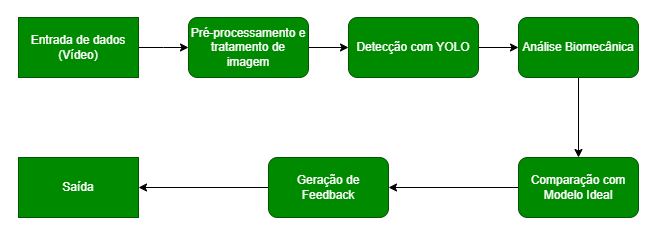
\includegraphics[width=0.75\linewidth]{resources/floats/ilustracoes/arquitetura.png}
    \end{flushleft}
    \addcontentsline{lof}{figure}{Ilustração X – Fluxograma da arquitetura do projeto}
\end{figura}
\FloatBarrier

O fluxograma é composto pelas seguintes ações:

\begin{myitemize}
    \item \textbf{Entrada de dados (Vídeo)}: O sistema recebe como entrada vídeos contendo arremessos no basquetebol, que serão utilizados como base para análise biomecânica.

    \item \textbf{Pré-processamento e tratamento de imagem}: Os quadros extraídos dos vídeos passam por processos de redimensionamento, filtragem e correção de contraste, preparando as imagens para a detecção com maior precisão.

    \item \textbf{Detecção com YOLO}: Utiliza-se o modelo YOLO para identificar automaticamente partes do corpo do atleta, como cabeça, ombros, cotovelos e mãos, em cada quadro analisado.

    \item \textbf{Análise Biomecânica}: A partir dos pontos detectados, são calculados ângulos articulares e características do movimento que representam a execução do arremesso.

    \item \textbf{Comparação com Modelo Ideal}: Os dados obtidos são comparados com uma referência ideal de arremesso, permitindo identificar falhas na técnica ou na postura do atleta.

    \item \textbf{Geração de Feedback}: Com base na comparação, o sistema fornece orientações visuais e textuais destacando o que pode ser aprimorado na execução do movimento.

    \item \textbf{Saída}: Os resultados são disponibilizados na forma de visualizações gráficas, imagens anotadas ou arquivos exportáveis, auxiliando treinadores e atletas no processo de correção e desempenho.
\end{myitemize}


\secao{Diagrama de Caso de Uso}

O diagrama de caso de uso apresentado na Ilustração 15 a seguir mostra as principais funcionalidades do Sistema de Análise de Arremessos sob a perspectiva do utilizador principal e as interações que este pode ter para atingir os seus objetivos.

\begin{figura}{Diagrama de Caso de Uso}{O Autor}
    \begin{flushleft}
        \label{fig:casouso}
        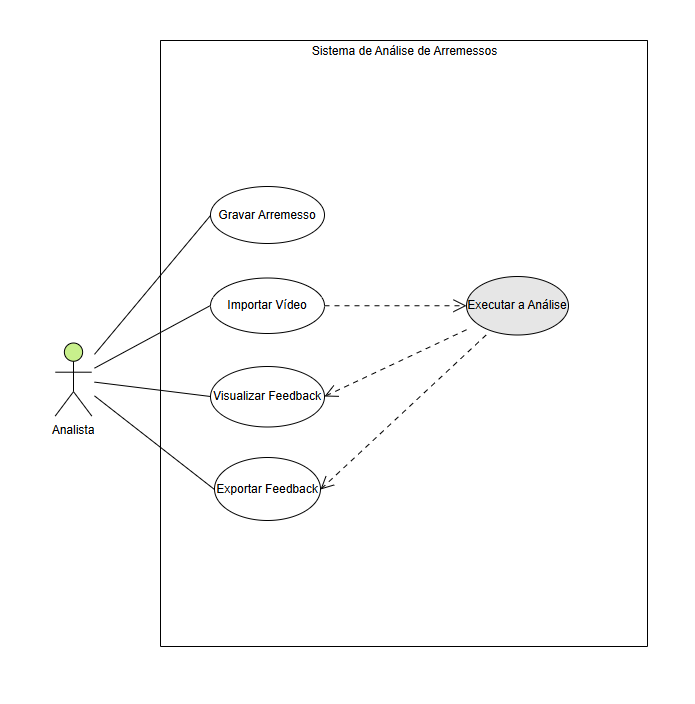
\includegraphics[width=0.70\linewidth]{resources/floats/ilustracoes/casouso.png}
    \end{flushleft}
    \addcontentsline{lof}{figure}{Ilustração X – Diagrama de Caso de Uso}
\end{figura}
\FloatBarrier

Como demonstrado no diagrama, o O \textbf{Analista}, que pode ser o treinador ou o próprio jogador que fez o arremesso, possui as seguintes ações dentro do sistema:

\begin{myitemize}
    \item \textbf{Gravar Arremesso}: Embora tecnicamente a gravação de vídeo possa ocorrer fora do sistema (por meio de câmeras ou dispositivos móveis), este caso de uso está presente como uma etapa inicial no fluxo de trabalho do Analista. Ele representa a captura do conteúdo necessário para alimentar o sistema de análise.

    \item \textbf{Importar Vídeo}: Após a gravação, o Analista realiza o upload do vídeo para o sistema. O vídeo deve conter um arremesso completo e estar em um formato compatível com os algoritmos de análise.

    \item \textbf{Executar a Análise}: Com o vídeo já carregado, o Analista pode solicitar que o sistema realize a análise biomecânica. Esse processo envolve múltiplas operações internas, como a detecção de pontos articulares via modelo YOLO, cálculo dos ângulos de movimento e comparação dos dados obtidos com um modelo ideal pré-estabelecido.

    \item \textbf{Visualizar Feedback}: Após a conclusão da análise, o Analista pode acessar os resultados gerados. O feedback inclui melhorias que o atleta pode buscar para melhorar a eficiência de seus arremessos.
    
    \item \textbf{Exportar Feedback}: Por fim, o Analista tem a possibilidade de exportar os dados gerados pelo sistema, para assim poder comparar os arremessos ao longo do tempo.
\end{myitemize}

\secao{Wireframes}

Os Wireframes a seguir mostram uma projeção do protótipo do sistema de análise.

\subsecao{Wireframe 1}

\begin{figura}{Wireframe 1}{O Autor}
    \begin{flushleft}
        \label{fig:wireframe1}
        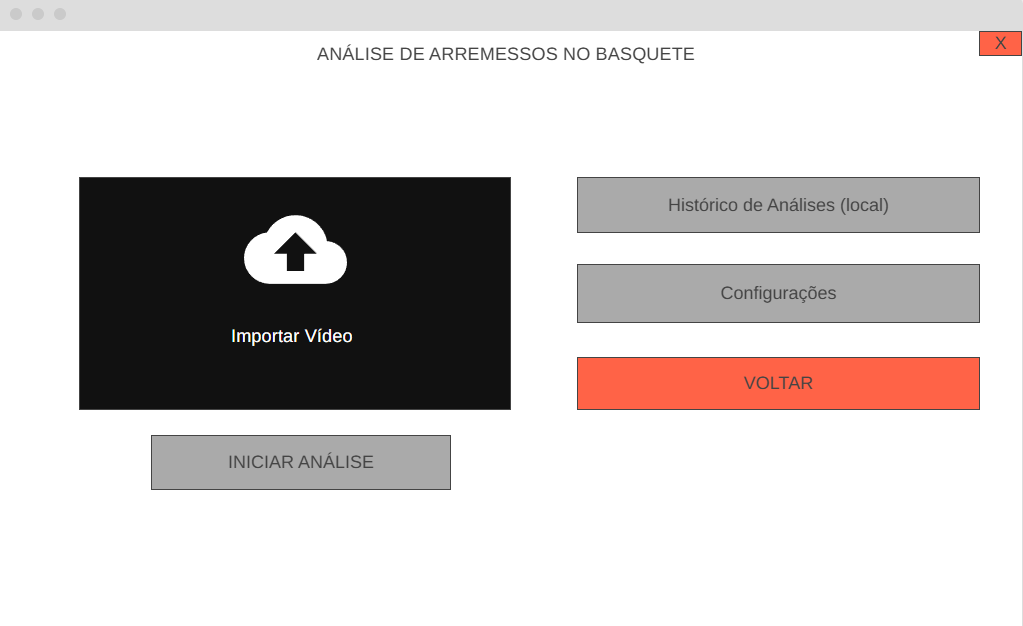
\includegraphics[width=0.69\linewidth]{resources/floats/ilustracoes/WIREFRAME1.png}
    \end{flushleft}
    \addcontentsline{lof}{figure}{Ilustração X – Wireframe 1}
\end{figura}
\FloatBarrier

O Wireframe mostrado na figura acima, descreve a tela inicial do protótipo, tendo como função principal importar o vídeo do arremesso, após a importação ao clicar no botão de análise, o modelo do YOLO entra em ação, fazendo o processamento do vídeo.
Além disso, temos a aba de configurações e também um botão para ver o histórico de análises, utilizando os registros que foram salvos localmente pelo usuário, por fim, um botão de fechar o sistema está disponível.

\subsecao{Wireframe 2}

\begin{figura}{Wireframe 2}{O Autor}
    \begin{flushleft}
        \label{fig:wireframe2}
        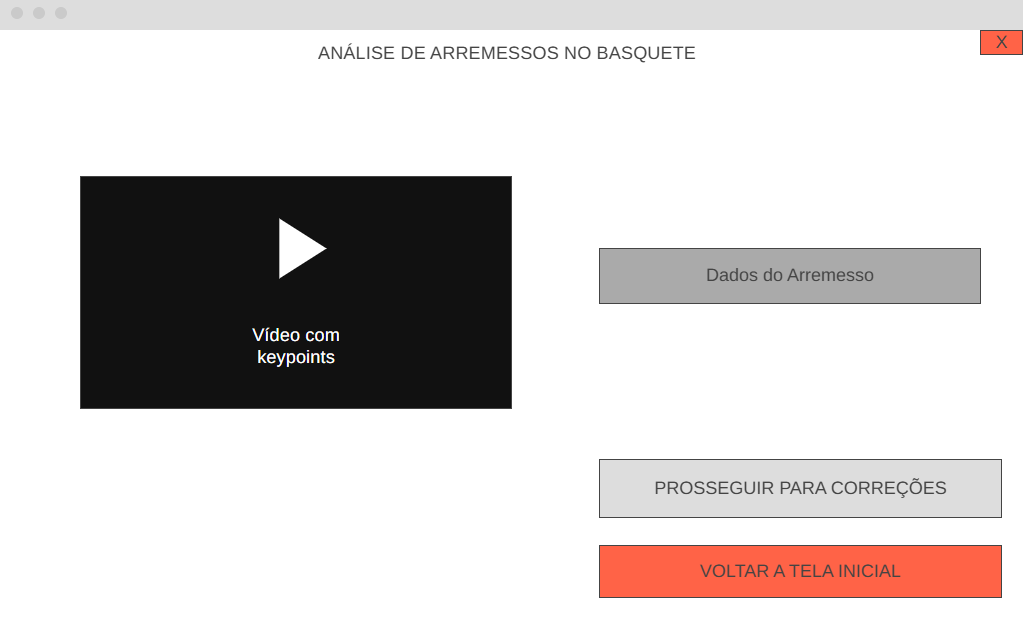
\includegraphics[width=0.69\linewidth]{resources/floats/ilustracoes/WIREFRAME2.png}
    \end{flushleft}
    \addcontentsline{lof}{figure}{Ilustração X – Wireframe 2}
\end{figura}
\FloatBarrier

Já o Wireframe 2 mostrado na figura acima, descreve a tela em que o vídeo processado aparece, com as métricas do arremesso aparecendo ao lado, além disso existe a opção de voltar ao menu principal e a opção de avançar para o feedback de melhorias do arremesso.

\subsecao{Wireframe 3}

\begin{figura}{Wireframe 3}{O Autor}
    \begin{flushleft}
        \label{fig:wireframe3}
        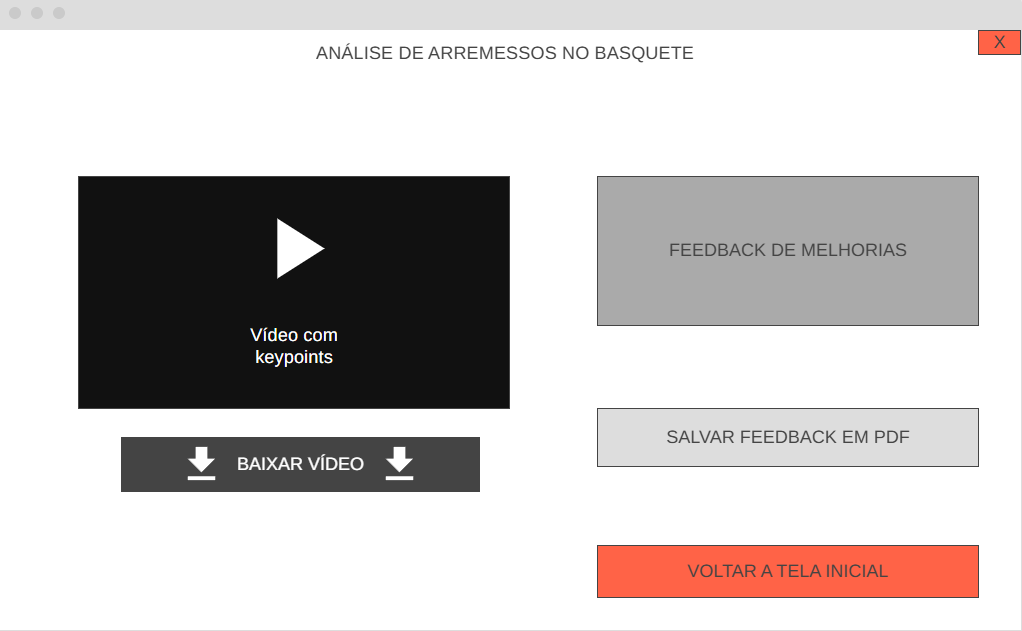
\includegraphics[width=0.69\linewidth]{resources/floats/ilustracoes/WIREFRAME3.png}
    \end{flushleft}
    \addcontentsline{lof}{figure}{Ilustração X – Wireframe 3}
\end{figura}
\FloatBarrier

Nesta parte, conseguimos novamente ver o vídeo, porém agora com o feedback de pontos a melhorar ao lado, caso o usuário ache necessário, existe a opção de exportar o vídeo e também o feedback em pdf, um botão de voltar ao menu principal após a conclusão da
análise está disponível, todas as abas tem um botão para fechar o programa também no canto superior direito da tela.
